%%%%%%%%%%%%%%%%%%%%%%%%%%%%%%%%%%%%%%%%%%%%%%%%%%%%%%%%%%%%%%%%%%%%%%%%%%%%%%%%
\subsection{Επισκόπηση}
\label{subsection:02_03_03:01}

Η δομή του συστήματος που προτείνουμε προς επίλυση του προβλήματος
\ref{prob:02_03:the_problem} δεδομένων των παραδοχών
\ref{assumption:02_03_01:01}, \ref{assumption:02_03_01:02}, και
\ref{assumption:02_03_01:03}, το οποίο συμβολίζεται με το ακρωνύμιο PGL-FMIC
(Passive Global Localisation---Fourier-Mellin Invariant matching with Centroids
for translation), απεικονίζεται στο σχήμα \ref{fig:02_03_03:overall_system}. Το
σύστημα απαιτεί ως είσοδο ένα διάνυσμα δισδιάστατων μετρήσεων $\mathcal{S}_R$,
το οποίο λαμβάνεται από τον αισθητήρα lidar του ρομπότ από την πραγματική του
στάση, τον χάρτη $\bm{M}$ του περιβάλλοντος του ρομπότ, και
τον αριθμό των υποθέσεων στάσης οι οποίες θα διασκοριστούν στον ελεύθερο
χώρο που οριοθετείται από τα σύνορα του χάρτη, $|\mathcal{H}|$.

Αρχικά παράγεται ένα σύνολο υποθέσεων στάσης $\mathcal{H} = \{\bm{h}_i\}$, $i =
\{0, 1, \dots, |\mathcal{H}|-1\}$ εντός του ελεύθερου χώρου του χάρτη, με
τυχαίο τρόπο. Οι περιεχόμενες στο σύνολο $\mathcal{H}$ στάσεις τοποθετούνται σε
μια ουρά $\bm{q}$, και εξάγονται σειριακά από αυτήν προτού εισαχθούν στη βασική
μέθοδο, η οποία συμβολίζεται με το ακρωνύμιο FMIC (αναλυτικότερα στις ενότητες
\ref{subsection:02_03_03:02} και \ref{subsection:02_03_03:03}). Η έξοδός της
αναφέρει μια εκτίμηση στάσης $\bm{h}_i^{\prime\prime}$ του ρομπότ, έναν
συντελεστή κλίμακας $\sigma_i$, και ένα μέτρο ομοιότητας $w_i$ για κάθε
εκτίμηση---το νόημα των δύο τελευταίων περιγράφεται λεπτομερώς στις ενότητες
\ref{subsec:01_01_02_7} και \ref{subsection:02_03_03:02}, και η χρησιμότητά
τους στην ενότητα \ref{subsection:02_03_03:04}. Οι τρεις έξοδοι ανά υπόθεση
αποθηκεύονται και, όταν αδειάσει η ουρά, η ολικά καταλληλότερη εκτίμηση στάσης
αναφέρεται ως η στάση του ρομπότ από το σύστημα. Αυτό γίνεται μέσω μιας
διαδικασίας διαλογής και κατάταξης η οποία απορρίπτει τις υποψήφιες εκτιμήσεις
στάσης του συνόλου $\{\bm{h}_i^{\prime\prime}\}$ με βάση τον αναφερόμενο
συντελεστή κλίμακας $\sigma_i$ προτού επιλέξει εκείνη της οποίας το μέτρο
ομοιότητας $w_i$ είναι το υψηλότερο μεταξύ όλων των υποψηφίων εκτιμήσεων
(ενότητα \ref{subsection:02_03_03:04}).

\begin{figure}[h]\centering
\tikzset{every picture/.style={line width=0.75pt}} %set default line width to 0.75pt

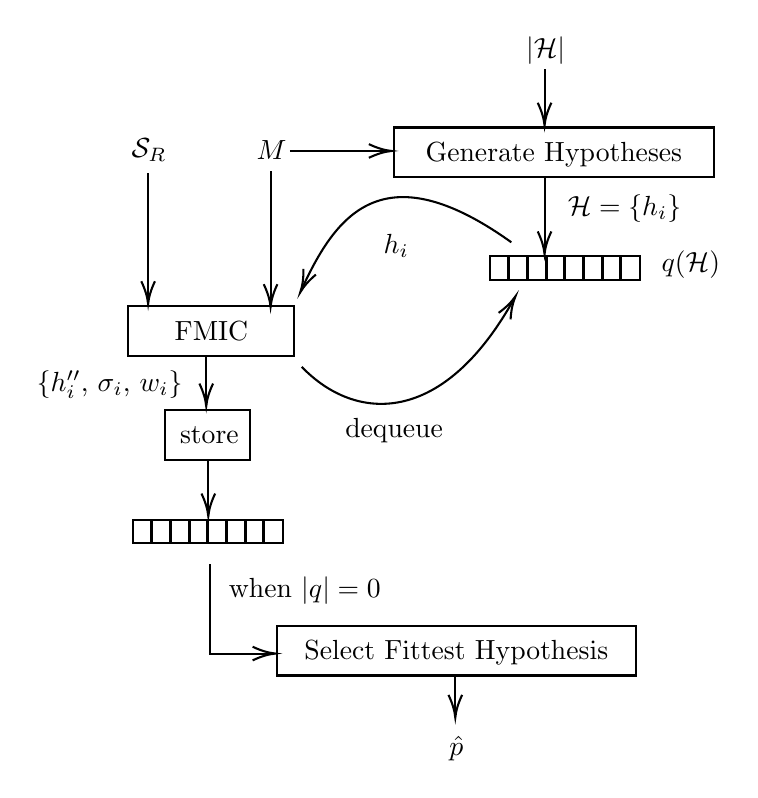
\begin{tikzpicture}[x=0.75pt,y=0.75pt,yscale=-1,xscale=1]
%uncomment if require: \path (0,447); %set diagram left start at 0, and has height of 447

%Straight Lines [id:da7180108526379969]
\draw    (108.5,68) -- (108.5,129) ;
\draw [shift={(108.5,131)}, rotate = 270] [color={rgb, 255:red, 0; green, 0; blue, 0 }  ][line width=0.75]    (10.93,-3.29) .. controls (6.95,-1.4) and (3.31,-0.3) .. (0,0) .. controls (3.31,0.3) and (6.95,1.4) .. (10.93,3.29)   ;
%Straight Lines [id:da03009202516620957]
\draw    (299.5,70) -- (299.5,86) -- (299.5,105) ;
\draw [shift={(299.5,107)}, rotate = 270] [color={rgb, 255:red, 0; green, 0; blue, 0 }  ][line width=0.75]    (10.93,-3.29) .. controls (6.95,-1.4) and (3.31,-0.3) .. (0,0) .. controls (3.31,0.3) and (6.95,1.4) .. (10.93,3.29)   ;
%Curve Lines [id:da7710107431830926]
\draw    (182.5,161.29) .. controls (208.37,188.15) and (250.58,190.27) .. (284.98,128.23) ;
\draw [shift={(285.5,127.29)}, rotate = 478.71] [color={rgb, 255:red, 0; green, 0; blue, 0 }  ][line width=0.75]    (10.93,-3.29) .. controls (6.95,-1.4) and (3.31,-0.3) .. (0,0) .. controls (3.31,0.3) and (6.95,1.4) .. (10.93,3.29)   ;
%Straight Lines [id:da8319074018571286]
\draw    (167.5,67) -- (167.5,120) -- (167.5,130.43) ;
\draw [shift={(167.5,132.43)}, rotate = 270] [color={rgb, 255:red, 0; green, 0; blue, 0 }  ][line width=0.75]    (10.93,-3.29) .. controls (6.95,-1.4) and (3.31,-0.3) .. (0,0) .. controls (3.31,0.3) and (6.95,1.4) .. (10.93,3.29)   ;
%Straight Lines [id:da9443063587697282]
\draw    (299.5,18) -- (299.5,34) -- (299.5,43) ;
\draw [shift={(299.5,45)}, rotate = 270] [color={rgb, 255:red, 0; green, 0; blue, 0 }  ][line width=0.75]    (10.93,-3.29) .. controls (6.95,-1.4) and (3.31,-0.3) .. (0,0) .. controls (3.31,0.3) and (6.95,1.4) .. (10.93,3.29)   ;
%Curve Lines [id:da9475685171094514]
\draw    (182.75,123.33) .. controls (198.68,89.07) and (221.06,56.63) .. (283.5,101.29) ;
\draw [shift={(181.79,125.43)}, rotate = 294.57] [color={rgb, 255:red, 0; green, 0; blue, 0 }  ][line width=0.75]    (10.93,-3.29) .. controls (6.95,-1.4) and (3.31,-0.3) .. (0,0) .. controls (3.31,0.3) and (6.95,1.4) .. (10.93,3.29)   ;
%Straight Lines [id:da7873103370093042]
\draw    (176.79,57.29) -- (223.79,57.29) ;
\draw [shift={(225.79,57.29)}, rotate = 180] [color={rgb, 255:red, 0; green, 0; blue, 0 }  ][line width=0.75]    (10.93,-3.29) .. controls (6.95,-1.4) and (3.31,-0.3) .. (0,0) .. controls (3.31,0.3) and (6.95,1.4) .. (10.93,3.29)   ;
%Shape: Rectangle [id:dp9316400431844878]
\draw   (273,108) -- (282.5,108) -- (282.5,119.29) -- (273,119.29) -- cycle ;
%Shape: Rectangle [id:dp2562271025125258]
\draw   (282,108) -- (291.5,108) -- (291.5,119.29) -- (282,119.29) -- cycle ;

%Shape: Rectangle [id:dp39303754153535886]
\draw   (291,108) -- (300.5,108) -- (300.5,119.29) -- (291,119.29) -- cycle ;
%Shape: Rectangle [id:dp6791562149193224]
\draw   (300,108) -- (309.5,108) -- (309.5,119.29) -- (300,119.29) -- cycle ;

%Shape: Rectangle [id:dp5956961748100666]
\draw   (309,108) -- (318.5,108) -- (318.5,119.29) -- (309,119.29) -- cycle ;
%Shape: Rectangle [id:dp03638414398094558]
\draw   (318,108) -- (327.5,108) -- (327.5,119.29) -- (318,119.29) -- cycle ;

%Shape: Rectangle [id:dp7241945812745509]
\draw   (327,108) -- (336.5,108) -- (336.5,119.29) -- (327,119.29) -- cycle ;
%Shape: Rectangle [id:dp30493977014241125]
\draw   (336,108) -- (345.5,108) -- (345.5,119.29) -- (336,119.29) -- cycle ;


%Straight Lines [id:da5492785297164644]
\draw    (256.5,310.29) -- (256.5,328.29) ;
\draw [shift={(256.5,330.29)}, rotate = 270] [color={rgb, 255:red, 0; green, 0; blue, 0 }  ][line width=0.75]    (10.93,-3.29) .. controls (6.95,-1.4) and (3.31,-0.3) .. (0,0) .. controls (3.31,0.3) and (6.95,1.4) .. (10.93,3.29)   ;
%Straight Lines [id:da8400249545776366]
\draw    (138.5,256.43) -- (138.5,299.43) -- (167.79,299.43) ;
\draw [shift={(169.79,299.43)}, rotate = 180] [color={rgb, 255:red, 0; green, 0; blue, 0 }  ][line width=0.75]    (10.93,-3.29) .. controls (6.95,-1.4) and (3.31,-0.3) .. (0,0) .. controls (3.31,0.3) and (6.95,1.4) .. (10.93,3.29)   ;
%Shape: Rectangle [id:dp36899940738692605]
\draw   (101,235) -- (110.5,235) -- (110.5,246.29) -- (101,246.29) -- cycle ;
%Shape: Rectangle [id:dp3740402995546943]
\draw   (110,235) -- (119.5,235) -- (119.5,246.29) -- (110,246.29) -- cycle ;

%Shape: Rectangle [id:dp9204771715668112]
\draw   (119,235) -- (128.5,235) -- (128.5,246.29) -- (119,246.29) -- cycle ;
%Shape: Rectangle [id:dp2611557502938522]
\draw   (128,235) -- (137.5,235) -- (137.5,246.29) -- (128,246.29) -- cycle ;

%Shape: Rectangle [id:dp5918549750705964]
\draw   (137,235) -- (146.5,235) -- (146.5,246.29) -- (137,246.29) -- cycle ;
%Shape: Rectangle [id:dp7742676605094942]
\draw   (146,235) -- (155.5,235) -- (155.5,246.29) -- (146,246.29) -- cycle ;

%Shape: Rectangle [id:dp4802635551676304]
\draw   (155,235) -- (164.5,235) -- (164.5,246.29) -- (155,246.29) -- cycle ;
%Shape: Rectangle [id:dp005738431700191393]
\draw   (164,235) -- (173.5,235) -- (173.5,246.29) -- (164,246.29) -- cycle ;


%Straight Lines [id:da2941675174511593]
\draw    (136.5,156.29) -- (136.5,178.29) ;
\draw [shift={(136.5,180.29)}, rotate = 270] [color={rgb, 255:red, 0; green, 0; blue, 0 }  ][line width=0.75]    (10.93,-3.29) .. controls (6.95,-1.4) and (3.31,-0.3) .. (0,0) .. controls (3.31,0.3) and (6.95,1.4) .. (10.93,3.29)   ;
%Straight Lines [id:da828241073247397]
\draw    (137.5,206.29) -- (137.5,231.29) ;
\draw [shift={(137.5,233.29)}, rotate = 270] [color={rgb, 255:red, 0; green, 0; blue, 0 }  ][line width=0.75]    (10.93,-3.29) .. controls (6.95,-1.4) and (3.31,-0.3) .. (0,0) .. controls (3.31,0.3) and (6.95,1.4) .. (10.93,3.29)   ;

% Text Node
\draw (109,57) node   [align=left] {$\mathcal{S}_R$};
% Text Node
\draw    (227,46) -- (381,46) -- (381,70) -- (227,70) -- cycle  ;
\draw (304,59) node   [align=left] {Generate Hypotheses};
% Text Node
\draw    (99,132) -- (179,132) -- (179,156) -- (99,156) -- cycle  ;
\draw (139,144) node   [align=left] {FMIC};
% Text Node
\draw (90,170) node   [align=left] {$\{\bm{h}_i^{\prime\prime}$, $\sigma_i$, $w_i\}$};
% Text Node
\draw (338,85) node   [align=left] {$\mathcal{H} = \{\bm{h}_i\}$};
% Text Node
\draw (168,57) node   [align=left] {$\bm{M}$};
% Text Node
\draw (228,103) node   [align=left] {$\bm{h}_i$};
% Text Node
\draw (227,192) node   [align=left] {dequeue};
% Text Node
\draw (300,9) node   [align=left] {$|\mathcal{H}|$};
% Text Node
\draw    (170.5,286) -- (343.5,286) -- (343.5,310) -- (170.5,310) -- cycle  ;
\draw (257,299) node   [align=left] {Select Fittest Hypothesis};
% Text Node
\draw (370,112) node   [align=left] {$\bm{q}(\mathcal{H})$};
% Text Node
\draw (184,269) node   [align=left] {when $|\bm{q}|=0$};
% Text Node
\draw (257,345) node   [align=left] {$\hat{\bm{p}}$};
% Text Node
\draw    (116.5,182) -- (157.5,182) -- (157.5,206) -- (116.5,206) -- cycle  ;
\draw (138,194) node   [align=left] {store};
\end{tikzpicture}
\caption{\small Η δομή του προτεινόμενου συστήματος PGL-FMIC επίλυσης του
         προβλήματος \ref{prob:02_03:the_problem}. Αφού δημιουργηθεί το σύνολο
         των υποθέσεων στάσης $\mathcal{H}$ και εισαχθεί στην ουρά $\bm{q}$, το
         περιεχόμενό της τροφοδοτείται ένα προς ένα στο σύστημα εκτίμησης των
         υποψηφίων στάσεων, FMIC, από το οποίο εξάγονται οι εκτιμήσεις στάσης
         $\bm{h}_i^{\prime\prime}$ και μετρικές της ποιότητας εκτίμησης
         $\sigma_i$ και $w_i$. Μετά το τέλος της επεξεργασίας όλων των υποθέσων
         στάσης αυτές οι μετρικές χρησιμεύουν για την εξαγωγή της τελικής
         εκτίμησης στάσης $\bm{\hat{p}}$ του ρομπότ από το σύστημα}
  \label{fig:02_03_03:overall_system}
\end{figure}

Το σχήμα \ref{fig:02_03_03:fmic} απεικονίζει την εσωτερική δομή της βασικής
μεθόδου που προτείνεται, ονομαζόμενη FMIC. Μόλις σε αυτήν εισαχθεί μια υπόθεση
$\bm{h}_i$, η μέθοδος προσπαθεί να εκτιμήσει πρώτα τον προσανατολισμό του
ρομπότ και στη συνέχεια τη θέση του σε σχέση με την υπόθεση, στο σύστημα
αναφοράς του χάρτη $\bm{M}$.


\begin{figure}[h]\centering
\tikzset{every picture/.style={line width=0.75pt}} %set default line width to 0.75pt

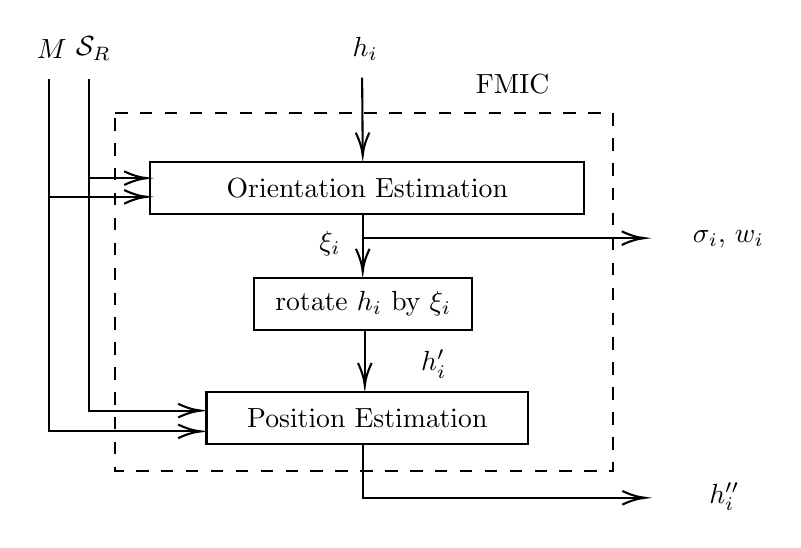
\begin{tikzpicture}[x=0.75pt,y=0.75pt,yscale=-1,xscale=1]
%uncomment if require: \path (0,300); %set diagram left start at 0, and has height of 300

%Straight Lines [id:da8451108171786026]
\draw    (271.5,76) -- (271.77,111.43) ;
\draw [shift={(271.79,113.43)}, rotate = 269.56] [color={rgb, 255:red, 0; green, 0; blue, 0 }  ][line width=0.75]    (10.93,-3.29) .. controls (6.95,-1.4) and (3.31,-0.3) .. (0,0) .. controls (3.31,0.3) and (6.95,1.4) .. (10.93,3.29)   ;
%Straight Lines [id:da4780501712403977]
\draw    (271.79,141.43) -- (271.79,167.43) ;
\draw [shift={(271.79,169.43)}, rotate = 270] [color={rgb, 255:red, 0; green, 0; blue, 0 }  ][line width=0.75]    (10.93,-3.29) .. controls (6.95,-1.4) and (3.31,-0.3) .. (0,0) .. controls (3.31,0.3) and (6.95,1.4) .. (10.93,3.29)   ;
%Straight Lines [id:da569100730417724]
\draw    (272.79,197.43) -- (272.79,222.43) ;
\draw [shift={(272.79,224.43)}, rotate = 270] [color={rgb, 255:red, 0; green, 0; blue, 0 }  ][line width=0.75]    (10.93,-3.29) .. controls (6.95,-1.4) and (3.31,-0.3) .. (0,0) .. controls (3.31,0.3) and (6.95,1.4) .. (10.93,3.29)   ;
%Straight Lines [id:da3942224067842923]
\draw    (271.79,252.43) -- (271.79,278.43) -- (405.79,278.43) ;
\draw [shift={(407.79,278.43)}, rotate = 180] [color={rgb, 255:red, 0; green, 0; blue, 0 }  ][line width=0.75]    (10.93,-3.29) .. controls (6.95,-1.4) and (3.31,-0.3) .. (0,0) .. controls (3.31,0.3) and (6.95,1.4) .. (10.93,3.29)   ;
%Straight Lines [id:da1656606324083285]
\draw    (139.79,76.43) -- (139.79,124.43) -- (165.79,124.43) ;
\draw [shift={(167.79,124.43)}, rotate = 180] [color={rgb, 255:red, 0; green, 0; blue, 0 }  ][line width=0.75]    (10.93,-3.29) .. controls (6.95,-1.4) and (3.31,-0.3) .. (0,0) .. controls (3.31,0.3) and (6.95,1.4) .. (10.93,3.29)   ;
%Straight Lines [id:da7481019832605267]
\draw    (120.79,76.43) -- (120.79,133.43) -- (165.79,133.43) ;
\draw [shift={(167.79,133.43)}, rotate = 180] [color={rgb, 255:red, 0; green, 0; blue, 0 }  ][line width=0.75]    (10.93,-3.29) .. controls (6.95,-1.4) and (3.31,-0.3) .. (0,0) .. controls (3.31,0.3) and (6.95,1.4) .. (10.93,3.29)   ;
%Straight Lines [id:da02254062670437551]
\draw    (120.79,133.43) -- (120.79,246.43) -- (191.79,246.43) ;
\draw [shift={(193.79,246.43)}, rotate = 180] [color={rgb, 255:red, 0; green, 0; blue, 0 }  ][line width=0.75]    (10.93,-3.29) .. controls (6.95,-1.4) and (3.31,-0.3) .. (0,0) .. controls (3.31,0.3) and (6.95,1.4) .. (10.93,3.29)   ;
%Straight Lines [id:da8105737578724599]
\draw    (139.79,115.43) -- (139.79,236.43) -- (191.79,236.43) ;
\draw [shift={(193.79,236.43)}, rotate = 180] [color={rgb, 255:red, 0; green, 0; blue, 0 }  ][line width=0.75]    (10.93,-3.29) .. controls (6.95,-1.4) and (3.31,-0.3) .. (0,0) .. controls (3.31,0.3) and (6.95,1.4) .. (10.93,3.29)   ;
%Shape: Rectangle [id:dp041152402740282534]
\draw  [dash pattern={on 4.5pt off 4.5pt}] (152.5,93) -- (392.33,93) -- (392.33,265.43) -- (152.5,265.43) -- cycle ;
%Straight Lines [id:da4152455210630952]
\draw    (271.79,153.33) -- (405.5,153.33) ;
\draw [shift={(407.5,153.33)}, rotate = 179.96] [color={rgb, 255:red, 0; green, 0; blue, 0 }  ][line width=0.75]    (10.93,-3.29) .. controls (6.95,-1.4) and (3.31,-0.3) .. (0,0) .. controls (3.31,0.3) and (6.95,1.4) .. (10.93,3.29)   ;

% Text Node
\draw (142,62) node   [align=left] {$\mathcal{S}_R$};
% Text Node
\draw (273,62) node   [align=left] {$\bm{h}_i$};
% Text Node
\draw (122,62) node   [align=left] {$\bm{M}$};
% Text Node
\draw    (169.5,116.5) -- (378.5,116.5) -- (378.5,141.5) -- (169.5,141.5) -- cycle  ;
\draw (274,129) node   [align=left] {Orientation Estimation};
% Text Node
\draw (256,156) node   [align=left] {$\xi_i$};
% Text Node
\draw    (219.5,172.5) -- (324.5,172.5) -- (324.5,197.5) -- (219.5,197.5) -- cycle  ;
\draw (272,185) node   [align=left] {rotate $\bm{h}_i$ by $\xi_i$};
% Text Node
\draw    (196.5,227.5) -- (351.5,227.5) -- (351.5,252.5) -- (196.5,252.5) -- cycle  ;
\draw (274,240) node   [align=left] {Position Estimation};
% Text Node
\draw (306,214) node   [align=left] {$\bm{h}_i^{\prime}$};
% Text Node
\draw (446,278) node   [align=left] {$\bm{h}_i^{\prime\prime}$};
% Text Node
\draw (448,154) node   [align=left] {$\sigma_i$, $w_i$};
% Text Node
\draw (344,79) node   [align=left] {FMIC};
\end{tikzpicture}
\caption{\small Η δομή της βασικής μεθόδου εκτίμησης στάσης του συστήματος
         PGL-FMIC, FMIC. Δεδομένου του χάρτη $\bm{M}$ του περιβάλλοντος του
         ρομπότ, της μέτρησης $\mathcal{S}_R$ από έναν πανοραμικό αισθητήρα
         δισδιάστατων μετρήσεων τύπου lidar που καταγράφεται από την
         πραγματική στάση του ρομπότ, και μια υπόθεση στάσης $\bm{h}_i$, πρώτα
         εκτελείται η εκτίμηση του προσανατολισμού $\xi_i$ του ρομπότ σε
         σχέση με την $\bm{h}_i$, και υπολογίζονται οι μετρικές $\sigma_i$,
         $w_i$, οι οποίες καθορίζουν την αξία της στάσης εξόδου
         $\bm{h}^{\prime\prime}$ ως μια υποψήφια στάση του ρομπότ. Στη συνέχεια
         προσδιορίζεται η θέση της εκτίμησης στάσης}
\label{fig:02_03_03:fmic}
\end{figure}


%%%%%%%%%%%%%%%%%%%%%%%%%%%%%%%%%%%%%%%%%%%%%%%%%%%%%%%%%%%%%%%%%%%%%%%%%%%%%%%%
\subsection{Εκτίμηση προσανατολισμού}
\label{subsection:02_03_03:02}

Δεδομένης μιας υπόθεσης στάσης $\bm{h}_i$, της μέτρησης $\mathcal{S}_R$ που
λαμβάνεται από τον πανοραμικό αισθητήρα δισδιάστατων μετρήσεων lidar, και του
χάρτη $\bm{M}$, το υποσύστημα εκτίμησης του προσανατολισμού του ρομπότ
(\textit{Orientation Estimation} στο σχήμα \ref{fig:02_03_03:fmic}) προσπαθεί να
εκτιμήσει (α) τον σχετικό προσανατολισμό του $\mathcal{S}_R$ σε σχέση με την
δισδιάστατη και ομοίως πανοραμική εικονική σάρωση που λαμβάνεται από την
υπόθεση στάσης $\bm{h}_i$, (β) τον συντελεστή κλίμακας μεταξύ των δύο σαρώσεων
$\sigma_i$, και (γ) ένα μέτρο της ομοιότητάς τους $w_i$.  Στο σχήμα
\ref{fig:02_03_03:estimate_orientation} απεικονίζονται οι εσωτερικές διεργασίες
του υποσυστήματος σε μορφή μπλοκ διαγράμματος.

Το υποσύστημα υπολογίζει πρώτα την εικονική σάρωση $\mathcal{S}_V^i$ από τη
στάση $\bm{h}_i$ εντός του χάρτη $\bm{M}$. Σε αυτό το σημείο είναι διαθέσιμες
δύο σαρώσεις: μία από τον φυσικό αισθητήρα του ρομπότ, η οποία έχει ληφθεί από
την πραγματική του στάση (ορισμός \ref{def:lidar}), και μία από έναν εικονικό
αισθητήρα, που καταγράφεται από την τυχαία στάση $\bm{h}_i$ (ορισμός
\ref{def:map_scan}). Στη συνέχεια τα τελικά σημεία των ακτίνων των δύο σαρώσεων
προβάλλονται στο επίπεδο $x-y$:
\begin{align}
  x_n &= x_0 + d_n \cos(\frac{2 \pi n}{N_s} - \pi + \theta_0) \label{eq:point_projection_x} \\
  y_n &= y_0 + d_n \sin(\frac{2 \pi n}{N_s} - \pi + \theta_0) \label{eq:point_projection_y}
\end{align}
όπου $(x_n,y_n)$ είναι οι συντεταγμένες του τελικού σημείου της ακτίνας $n$, $n
= \{0,1,\dots, N_s-1\}$, $d_n$ η μέτρηση απόστασης που αφορά στην ακτίνα $n$,
και $N_s$ ο αριθμός των ακτίνων που εκπέμπονται από τον αισθητήρα lidar.  Το
διάνυσμα $(x_0,y_0,\theta_0) \triangleq (0,0,0)$, δηλαδή τα τελικά σημεία και
των δύο σαρώσεων προβάλλονται στο τοπικό σύστημα συντεταγμένων του κάθε
αισθητήρα.  Από τη διαδικασία προβολής των δύο σαρώσεων προκύπτουν δύο σύνολα
σημείων στον δισδιάστατο χώρο, $\mathcal{P}_R$ και $\mathcal{P}_V^i$.  Τα
σύνολα σημείων $\mathcal{P}_R$ και $\mathcal{P}_V^i$ υπόκεινται στη συνέχεια σε
διακριτοποίηση με ένα σταθερό μέγεθος πλέγματος $N_G \times N_G$ (το οποίο
συνιστάται να είναι δύναμη του δύο: $N_G = 2^c$, όπου $c \in \mathbb{Z}^{+}$,
λόγω της αποτελεσματικότητας του FFT στην εκτέλεση πράξεων με πίνακες δύο
διαστάσεων των οποίων το μέγεθος είναι δύναμη του δύο \cite{Bulow2010}), η
οποία παράγει τα δισδιάστατα πλέγματα-εικόνες $\bm{r}$ και $\bm{v}_i$
αντίστοιχα. Τα πλέγματα αυτά στη συνέχεια εισάγονται στη διαδικασία FMI-SPOMF
(αλγόριθμος \ref{alg:image_registration}), η οποία εξάγει τη γωνία περιστροφής
$\xi_i$, τον συντελεστή κλίμακας $\sigma_i$, και το μέτρο ομοιότητας $w_i$
μεταξύ των δύο εικόνων $\bm{r}$ και $\bm{v}_i$, και συνεπώς μεταξύ των σαρώσεων
$\mathcal{S}_R$ και $\mathcal{S}_V^i$.


\begin{figure}[h]\centering
\tikzset{every picture/.style={line width=0.75pt}} %set default line width to 0.75pt
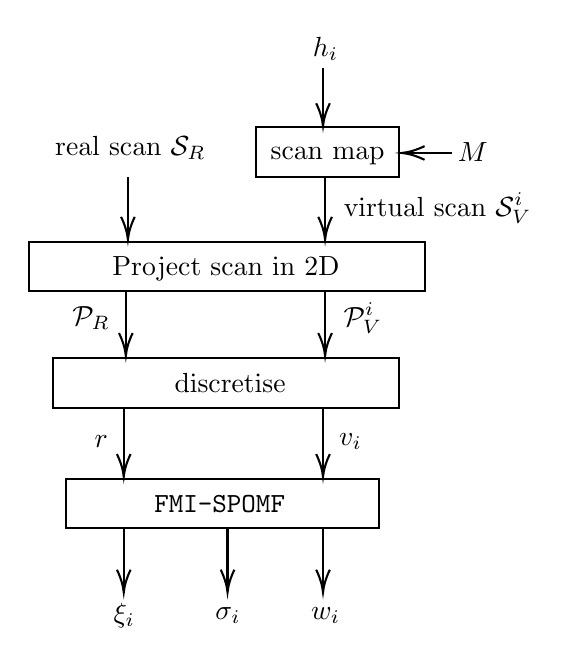
\begin{tikzpicture}[x=0.75pt,y=0.75pt,yscale=-1,xscale=1]
%uncomment if require: \path (0,392); %set diagram left start at 0, and has height of 392
%Straight Lines [id:da9730227266707869]
\draw    (235.79,104) -- (235.79,132) ;
\draw [shift={(235.79,134)}, rotate = 270] [color={rgb, 255:red, 0; green, 0; blue, 0 }  ][line width=0.75]    (10.93,-3.29) .. controls (6.95,-1.4) and (3.31,-0.3) .. (0,0) .. controls (3.31,0.3) and (6.95,1.4) .. (10.93,3.29)   ;
%Straight Lines [id:da2844027535234337]
\draw    (234.79,159) -- (234.79,188) ;
\draw [shift={(234.79,190)}, rotate = 270] [color={rgb, 255:red, 0; green, 0; blue, 0 }  ][line width=0.75]    (10.93,-3.29) .. controls (6.95,-1.4) and (3.31,-0.3) .. (0,0) .. controls (3.31,0.3) and (6.95,1.4) .. (10.93,3.29)   ;
%Straight Lines [id:da7071701796034313]
\draw    (330.79,159) -- (330.79,188) ;
\draw [shift={(330.79,190)}, rotate = 270] [color={rgb, 255:red, 0; green, 0; blue, 0 }  ][line width=0.75]    (10.93,-3.29) .. controls (6.95,-1.4) and (3.31,-0.3) .. (0,0) .. controls (3.31,0.3) and (6.95,1.4) .. (10.93,3.29)   ;
%Straight Lines [id:da8188669244663311]
\draw    (233.79,215) -- (233.79,246.29) ;
\draw [shift={(233.79,248.29)}, rotate = 270] [color={rgb, 255:red, 0; green, 0; blue, 0 }  ][line width=0.75]    (10.93,-3.29) .. controls (6.95,-1.4) and (3.31,-0.3) .. (0,0) .. controls (3.31,0.3) and (6.95,1.4) .. (10.93,3.29)   ;
%Straight Lines [id:da9321940706140008]
\draw    (329.79,215) -- (329.79,246.29) ;
\draw [shift={(329.79,248.29)}, rotate = 270] [color={rgb, 255:red, 0; green, 0; blue, 0 }  ][line width=0.75]    (10.93,-3.29) .. controls (6.95,-1.4) and (3.31,-0.3) .. (0,0) .. controls (3.31,0.3) and (6.95,1.4) .. (10.93,3.29)   ;
%Straight Lines [id:da6399429499252802]
\draw    (233.79,273) -- (233.79,302) ;
\draw [shift={(233.79,304)}, rotate = 270] [color={rgb, 255:red, 0; green, 0; blue, 0 }  ][line width=0.75]    (10.93,-3.29) .. controls (6.95,-1.4) and (3.31,-0.3) .. (0,0) .. controls (3.31,0.3) and (6.95,1.4) .. (10.93,3.29)   ;
%Straight Lines [id:da35220350679263834]
\draw    (329.79,273) -- (329.79,302) ;
\draw [shift={(329.79,304)}, rotate = 270] [color={rgb, 255:red, 0; green, 0; blue, 0 }  ][line width=0.75]    (10.93,-3.29) .. controls (6.95,-1.4) and (3.31,-0.3) .. (0,0) .. controls (3.31,0.3) and (6.95,1.4) .. (10.93,3.29)   ;
%Straight Lines [id:da3644508060580869]
\draw    (283.79,273) -- (283.79,302) ;
\draw [shift={(283.79,304)}, rotate = 270] [color={rgb, 255:red, 0; green, 0; blue, 0 }  ][line width=0.75]    (10.93,-3.29) .. controls (6.95,-1.4) and (3.31,-0.3) .. (0,0) .. controls (3.31,0.3) and (6.95,1.4) .. (10.93,3.29)   ;
%Straight Lines [id:da9423217519316076]
\draw    (329.79,51.29) -- (329.79,77.29) ;
\draw [shift={(329.79,79.29)}, rotate = 270] [color={rgb, 255:red, 0; green, 0; blue, 0 }  ][line width=0.75]    (10.93,-3.29) .. controls (6.95,-1.4) and (3.31,-0.3) .. (0,0) .. controls (3.31,0.3) and (6.95,1.4) .. (10.93,3.29)   ;
%Straight Lines [id:da39994064933770224]
\draw    (391.79,92.29) -- (369.79,92.29) ;
\draw [shift={(367.79,92.29)}, rotate = 360] [color={rgb, 255:red, 0; green, 0; blue, 0 }  ][line width=0.75]    (10.93,-3.29) .. controls (6.95,-1.4) and (3.31,-0.3) .. (0,0) .. controls (3.31,0.3) and (6.95,1.4) .. (10.93,3.29)   ;
%Shape: Rectangle [id:dp8211341324978452]
\draw   (356.79,249.29) -- (206,249.29) -- (206,273) -- (356.79,273) -- cycle ;
%Straight Lines [id:da22704241323955765]
\draw    (330.79,104) -- (330.79,132) ;
\draw [shift={(330.79,134)}, rotate = 270] [color={rgb, 255:red, 0; green, 0; blue, 0 }  ][line width=0.75]    (10.93,-3.29) .. controls (6.95,-1.4) and (3.31,-0.3) .. (0,0) .. controls (3.31,0.3) and (6.95,1.4) .. (10.93,3.29)   ;

% Text Node
% Text Node
\draw    (297.5,80) -- (366.5,80) -- (366.5,104) -- (297.5,104) -- cycle  ;
\draw (332,94) node   [align=left] {scan map};
% Text Node
\draw (331,42) node   [align=left] {$\bm{h}_i$};
% Text Node
\draw (402,92) node   [align=left] {$\bm{M}$};
% Text Node
\draw (237,90) node   [align=left] {real scan $\mathcal{S}_R$};
% Text Node
\draw (385,119) node   [align=left] {virtual scan $\mathcal{S}_V^i$};
% Text Node
\draw (218,172) node   [align=left] {$\mathcal{P}_R$};
% Text Node
\draw (349,172) node   [align=left] {$\mathcal{P}_V^i$};
% Text Node
% Text Node
\draw (280,261.29) node   [align=left] {\texttt{FMI-SPOMF}};
% Text Node
\draw (223,231.29) node   [align=left] {$\bm{r}$};
% Text Node
\draw (343,231.29) node   [align=left] {$\bm{v}_i$};
% Text Node
\draw (234,315.29) node   [align=left] {$\xi_i$};
% Text Node
\draw (284,315.29) node   [align=left] {$\sigma_i$};
% Text Node
\draw (331,315.29) node   [align=left] {$w_i$};
% Text Node
\draw    (188,135) -- (379,135) -- (379,159) -- (188,159) -- cycle  ;
\draw (283,148) node   [align=left] {Project scan in 2D};
% Text Node
\draw    (199.5,191) -- (366.5,191) -- (366.5,215) -- (199.5,215) -- cycle  ;
\draw (285,203) node   [align=left] {discretise};
\end{tikzpicture}
\caption{\small Η εσωτερική δομή του υποσυστήματος εκτίμησης περιστροφής και
         κλίμακας του συστήματος FMIC (σχήμα \ref{fig:02_03_03:fmic})}
\label{fig:02_03_03:estimate_orientation}
\end{figure}


Η εφαρμοσιμότητα του FMI-SPOMF σε σχέση με τις διακριτοποιημένες εκδόσεις των
συνόλων σημείων $\mathcal{P}_R$ και $\mathcal{P}_V^i$ είναι εφικτή και
έγκυρη τόσο στην περίπτωση όπου μια υπόθεση στάσης βρίσκεται κοντά στην
πραγματική στάση του ρομπότ, όσο και σε αυτήν που αυτό δεν ισχύει:

\begin{itemize}
  \item Στην πρώτη περίπτωση τα δύο σύνολα σημείων αποτελούνται
        από μία πλειοψηφία από σημεία που αντιπροσωπεύουν τμήματα του
        περιβάλλοντος/χάρτη που είναι ορατά και από τις δύο στάσεις, και από μία
        μειοψηφία σημείων που είναι ορατά αποκλειστικά από τη μία αλλά όχι από
        την άλλη. Αυτό το γεγονός αποδίδεται αποκλειστικά στη μετατόπιση της
        θέσης της υπόθεσης σε σχέση με την πραγματική θέση του ρομπότ. Τα
        σημεία της πρώτης κατηγορίας σχετίζονται μεταξύ τους μέσω
        μετατόπισης και περιστροφής λόγω της αναπαράστασης του περιβάλλοντος
        σε χάρτη (με την κλίμακα να παίζει ρόλο, η βαρύτητα του οποίου είναι
        αντιστρόφως ανάλογη της ανάλυσης του χάρτη). Τα σημεία της
        δεύτερης κατηγορίας μπορούν να θεωρηθούν ως θόρυβος ή μη γραμμικές
        παραμορφώσεις, έχοντας έτσι φθίνουσα επίδραση στο μέτρο ομοιότητας
        μεταξύ των εικόνων που αντιστοιχούν στα δύο σύνολα σημείων. Ανεξάρτητα
        από αυτό το είδος της ασυμφωνίας, η ομοιότητα μεταξύ των δύο εικόνων
        και η ποιότητα της εκτίμησης της μετατόπισης, περιστροφής, και κλίμακας,
        είναι ανάλογες με το ποσοστό των σημείων της πρώτης κατηγορίας σε
        σχέση με εκείνο της δεύτερης---ένα αποτέλεσμα που σε μεγάλο βαθμό
        αποδίδεται στην τεκμηριωμένη ευρωστία του FMI-SPOMF
        \cite{Qin-ShengChen1994a}.
  \item Στην δεύτερη περίπτωση η έξοδος των αλγορίθμων \ref{alg:spomf} και
        \ref{alg:image_registration}, και, κυρίως, η τιμή του μέτρου ομοιότητας
        $w$ είναι αυθαίρετες---ωστόσο, αν μια δεύτερη υπόθεση στάσης τυγχάνει να
        βρίσκεται πλησίον της πραγματικής στάσης του ρομπότ, τότε, επιπροσθέτως,
        το μέτρο ομοιότητας που αφορά στην πρώτη (λανθασμένη) υπόθεση είναι
        μικρότερο σε μέγεθος από εκείνο της δεύτερης, καθιστώντας έτσι εφικτή
        τη διάκριση μεταξύ των δύο.
\end{itemize}

Παρόλο που ο FMI-SPOMF είναι σε θέση να εξάγει τη μετατόπιση μεταξύ δύο
εικόνων, το γεγονός ότι στα συμφραζόμενα του κεφαλαίου (α) αυτές έχουν ληφθεί
από το τοπικό σύστημα αναφοράς κάθε αισθητήρα, και (β) η πραγματική θέση του
ρομπότ είναι άγνωστη---αυτά τα δύο καθιστούν το εξαγώμενο διάνυσμα μετατόπισης
χωρίς φυσική σημασία. Ωστόσο, εάν η υπόθεση στάσης $\bm{h}_i$ βρίσκεται σε μία
γειτονιά της πραγματικής θέσης του ρομπότ, αφού περιστραφεί κατά
$\xi_i$, μπορεί να εξαχθεί μια εκτίμηση της μετατόπισής της σε σχέση με την
πραγματική του στάση. Η διαδικασία διόρθωσης της θέσης περιγράφεται στην ενότητα
\ref{subsection:02_03_03:03}.


%%%%%%%%%%%%%%%%%%%%%%%%%%%%%%%%%%%%%%%%%%%%%%%%%%%%%%%%%%%%%%%%%%%%%%%%%%%%%%%%
\subsection{Εκτίμηση θέσης}
\label{subsection:02_03_03:03}

Μετά την περιστροφή της υπόθεσης $\bm{h}_i$ κατά τη γωνία που υπολογίστηκε από
το υποσύστημα εκτίμησης προσανατολισμού $\xi_i$, η προκύπτουσα στάση-υπόθεση, η
οποία συμβολίζεται στη συνέχεια με $\bm{h}_i^\prime$, εισάγεται στο υποσύστημα
εκτίμησης θέσης, το μπλοκ διάγραμμα του οποίου απεικονίζεται στο σχήμα
\ref{fig:02_03_03:estimate_position}.  Δεδομένης της περιεστραμμένης
υπόθεσης στάσης $\bm{h}_i^\prime$, της μέτρησης $\mathcal{S}_R$ που λαμβάνεται
από τον πανοραμικό αισθητήρα δισδιάστατων μετρήσεων lidar, και του χάρτη
$\bm{M}$, το υποσύστημα εκτίμησης της θέσης του ρομπότ (\textit{Position
Estimation} στο σχήμα \ref{fig:02_03_03:fmic}) προσπαθεί να εκτιμήσει τη
σχετική θέση του $\mathcal{S}_R$ σε σχέση με την δισδιάστατη και ομοίως
πανοραμική εικονική σάρωση που λαμβάνεται από την υπόθεση στάσης
$\bm{h}_i^\prime$.

\begin{figure}[h]\centering
\tikzset{every picture/.style={line width=0.75pt}} %set default line width to 0.75pt
  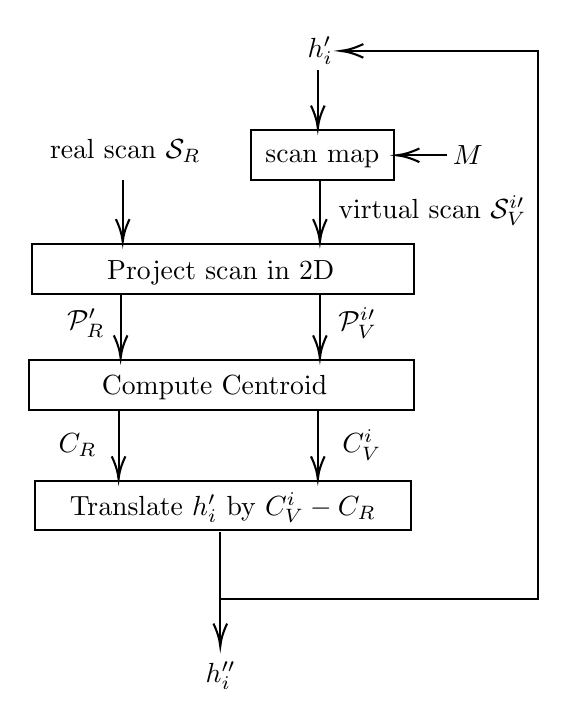
\begin{tikzpicture}[x=0.75pt,y=0.75pt,yscale=-1,xscale=1]
  %uncomment if require: \path (0,445); %set diagram left start at 0, and has height of 445

  %Straight Lines [id:da4890828235090363]
  \draw    (255.79,78.71) -- (255.79,106.71) ;
  \draw [shift={(255.79,108.71)}, rotate = 270] [color={rgb, 255:red, 0; green, 0; blue, 0 }  ][line width=0.75]    (10.93,-3.29) .. controls (6.95,-1.4) and (3.31,-0.3) .. (0,0) .. controls (3.31,0.3) and (6.95,1.4) .. (10.93,3.29)   ;
  %Straight Lines [id:da6287498008177574]
  \draw    (254.79,133.71) -- (254.79,162.71) ;
  \draw [shift={(254.79,164.71)}, rotate = 270] [color={rgb, 255:red, 0; green, 0; blue, 0 }  ][line width=0.75]    (10.93,-3.29) .. controls (6.95,-1.4) and (3.31,-0.3) .. (0,0) .. controls (3.31,0.3) and (6.95,1.4) .. (10.93,3.29)   ;
  %Straight Lines [id:da6679606992950171]
  \draw    (350.79,133.71) -- (350.79,162.71) ;
  \draw [shift={(350.79,164.71)}, rotate = 270] [color={rgb, 255:red, 0; green, 0; blue, 0 }  ][line width=0.75]    (10.93,-3.29) .. controls (6.95,-1.4) and (3.31,-0.3) .. (0,0) .. controls (3.31,0.3) and (6.95,1.4) .. (10.93,3.29)   ;
  %Straight Lines [id:da3250853238606073]
  \draw    (253.79,189.71) -- (253.79,221) ;
  \draw [shift={(253.79,223)}, rotate = 270] [color={rgb, 255:red, 0; green, 0; blue, 0 }  ][line width=0.75]    (10.93,-3.29) .. controls (6.95,-1.4) and (3.31,-0.3) .. (0,0) .. controls (3.31,0.3) and (6.95,1.4) .. (10.93,3.29)   ;
  %Straight Lines [id:da8663761783629615]
  \draw    (349.79,189.71) -- (349.79,221) ;
  \draw [shift={(349.79,223)}, rotate = 270] [color={rgb, 255:red, 0; green, 0; blue, 0 }  ][line width=0.75]    (10.93,-3.29) .. controls (6.95,-1.4) and (3.31,-0.3) .. (0,0) .. controls (3.31,0.3) and (6.95,1.4) .. (10.93,3.29)   ;
  %Straight Lines [id:da9085545032858575]
  \draw    (349.79,26) -- (349.79,52) ;
  \draw [shift={(349.79,54)}, rotate = 270] [color={rgb, 255:red, 0; green, 0; blue, 0 }  ][line width=0.75]    (10.93,-3.29) .. controls (6.95,-1.4) and (3.31,-0.3) .. (0,0) .. controls (3.31,0.3) and (6.95,1.4) .. (10.93,3.29)   ;
  %Straight Lines [id:da9263178883490375]
  \draw    (411.79,67) -- (389.79,67) ;
  \draw [shift={(387.79,67)}, rotate = 360] [color={rgb, 255:red, 0; green, 0; blue, 0 }  ][line width=0.75]    (10.93,-3.29) .. controls (6.95,-1.4) and (3.31,-0.3) .. (0,0) .. controls (3.31,0.3) and (6.95,1.4) .. (10.93,3.29)   ;
  %Straight Lines [id:da1800828112430095]
  \draw    (350.79,78.71) -- (350.79,106.71) ;
  \draw [shift={(350.79,108.71)}, rotate = 270] [color={rgb, 255:red, 0; green, 0; blue, 0 }  ][line width=0.75]    (10.93,-3.29) .. controls (6.95,-1.4) and (3.31,-0.3) .. (0,0) .. controls (3.31,0.3) and (6.95,1.4) .. (10.93,3.29)   ;
  %Straight Lines [id:da15117671546600464]
  \draw    (302.79,248.71) -- (302.79,280.71) -- (455.79,280.71) -- (455.79,16.71) -- (362.79,16.71) ;
  \draw [shift={(360.79,16.71)}, rotate = 360] [color={rgb, 255:red, 0; green, 0; blue, 0 }  ][line width=0.75]    (10.93,-3.29) .. controls (6.95,-1.4) and (3.31,-0.3) .. (0,0) .. controls (3.31,0.3) and (6.95,1.4) .. (10.93,3.29)   ;
  %Straight Lines [id:da9123253075624222]
  \draw    (302.79,280.71) -- (302.79,301.57) ;
  \draw [shift={(302.79,303.57)}, rotate = 270] [color={rgb, 255:red, 0; green, 0; blue, 0 }  ][line width=0.75]    (10.93,-3.29) .. controls (6.95,-1.4) and (3.31,-0.3) .. (0,0) .. controls (3.31,0.3) and (6.95,1.4) .. (10.93,3.29)   ;

  % Text Node
  \draw  (317.5,54.71) -- (386.5,54.71) -- (386.5,78.71) -- (317.5,78.71) -- cycle  ;
  \draw (352,68.71) node   [align=left] {scan map};
  % Text Node
  \draw (351,16.71) node   [align=left] {$\bm{h}_i^{\prime}$};
  % Text Node
  \draw (422,66.71) node   [align=left] {$\bm{M}$};
  % Text Node
  \draw (257,64.71) node   [align=left] {real scan $\mathcal{S}_R$};
  % Text Node
  \draw (405,93.71) node   [align=left] {virtual scan $\mathcal{S}_V^{i\prime}$};
  % Text Node
  \draw (238,147.71) node   [align=left] {$\mathcal{P}_R^\prime$};
  % Text Node
  \draw (369,147.71) node   [align=left] {$\mathcal{P}_V^{i\prime}$};
  % Text Node
  \draw (212,109.71) -- (396,109.71) -- (396,133.71) -- (212,133.71) -- cycle  ;
  \draw (303,123.71) node   [align=left] {Project scan in 2D};
  % Text Node
  \draw  (210.5,165.71) -- (396,165.71) -- (396,189.71) -- (210.5,189.71) -- cycle  ;
  \draw (300,178.71) node   [align=left] {Compute Centroid};
  % Text Node
  \draw (234,206.71) node   [align=left] {$\bm{C}_R$};
  % Text Node
  \draw (371,206.71) node   [align=left] {$\bm{C}_V^i$};
  % Text Node
  \draw (213.5,223.71) -- (394.5,223.71) -- (394.5,247.71) -- (213.5,247.71) -- cycle  ;
  \draw (304,236.71) node   [align=left] {Translate $\bm{h}_i^\prime$ by $\bm{C}_V^i - \bm{C}_R$};
  % Text Node
  \draw (303,317.57) node   [align=left] {$\bm{h}_i^{\prime\prime}$};
  \end{tikzpicture}
\caption{\small Η εσωτερική δομή του υποσυστήματος εκτίμησης θέσης του
         συστήματος FMIC (σχήμα \ref{fig:02_03_03:fmic})}
\label{fig:02_03_03:estimate_position}
\end{figure}

Αρχικά υπολογίζεται μια νέα σάρωση χάρτη $\mathcal{S}_V^{i\prime}$ από τη
διορθωμένη κατά γωνία υπόθεση στάσης $\bm{h}_i^\prime$. Τα τελικά της σημεία,
μαζί με εκείνα του διανύσματος μέτρησης του φυσικού αισθητήρα $\mathcal{S}_R$,
προβάλλονται εκ νέου στο επίπεδο $x-y$, με τη χρήση των εξισώσεων
(\ref{eq:point_projection_x}) και (\ref{eq:point_projection_y}). Σε αυτές τις
εξισώσεις, έχοντας ήδη εκτιμήσει τον προσανατολισμό του ρομπότ, η τιμή της
μεταβλητής $\theta_0$ αντικαθίσταται από την εκτίμηση προσανατολισμού του,
$\theta_{\bm{h}_i^\prime} = \theta_{\bm{h}_i} + \xi_i$. Τα δύο σύνολα σημείων
που προκύπτουν, $\mathcal{P}_R^\prime$ και $\mathcal{P}_V^{i\prime}$, είναι
τώρα ευθυγραμμισμένα ως προς τον προσανατολισμό, και κεντραρισμένα γύρω από την
αρχή $O(0,0)$. Στη συνέχεια υπολογίζεται το κεντροειδές κάθε πολυγώνου με
κορυφές $\mathcal{P}_R^\prime$ και $\mathcal{P}_V^{i\prime}$ μέσω των εξισώσεων
(\ref{eq:centroid_x}) και (\ref{eq:centroid_y}). Η θέση της υπόθεσης στάσης
$\bm{h}_i^\prime$ διορθώνεται στη συνέχεια με την πρόσθεση σε αυτήν της
διαφοράς θέσης μεταξύ των δύο κεντροειδών $\bm{C}_V^i$ και $\bm{C}_R$, και η
διαδικασία αυτή επαναλαμβάνεται έως ότου επιτευχθεί σύγκλιση ή συμπληρωθεί ένας
μέγιστος αριθμός επαναλήψεων. Εάν η θέση της υπόθεσης $\bm{h}_i^\prime$
βρίσκεται σε μία γειτονιά της πραγματικής θέσης του ρομπότ, τότε η διαφορά των
συντεταγμένων των κεντροειδών προσεγγίζει τη διαφορά των δύο αυτών
θέσεων---λόγω των παρατηρήσεων \ref{remark:smsm_benefit} και
\ref{remark:centroid_uniqueness}---συν κάποια επιπρόσθετη μετατόπιση που
προκαλείται από τα σημεία τα οποία είναι ορατά από τη μία θέση αλλά όχι από την
άλλη. Αυτό οφείλεται και πάλι στο γεγονός ότι διαφορετικά μέρη του
περιβάλλοντος/χάρτη καθίστανται (μη) ορατά από διαφορετικές θέσεις. Αντιθέτως,
εάν η υπόθεση $\bm{h}_i$ δεν είναι ορθή, η θέση της υπόθεσης $\bm{h}_i^\prime$
θα μετατοπιστεί σε μία τυχαία θέση. Η έξοδος της παραπάνω διαδικασίας είναι η
τελική εκτίμηση της στάσης $\bm{h}_i^{\prime\prime}$.


%%%%%%%%%%%%%%%%%%%%%%%%%%%%%%%%%%%%%%%%%%%%%%%%%%%%%%%%%%%%%%%%%%%%%%%%%%%%%%%%
\subsection{Επιλογή βέλτιστης υπόθεσης}
\label{subsection:02_03_03:04}

Μετά την επεξεργασία του συνόλου των υποθέσεων $\mathcal{H}$ έχει εξαχθεί μια
συλλογή από ίσες σε αριθμό τριπλέτες $\{\bm{h}_i^{\prime\prime}, \sigma_i,
w_i\}$, $i = 0,1,\dots,|\mathcal{H}|-1$. Προκειμένου να προσδιοριστεί η τελική
εκτίμηση της στάσης του ρομπότ θα πρέπει η εκτίμηση της κάθεμίας να αξιολογηθεί
ως προς τις μετρικές ευθυγράμμισης που εξήχθησαν κατά την εκτίμηση του
προσανατολισμού της υπόθεσης $\bm{h}_i$.  Θεωρητικά, για την πλησιέστερη στο
ρομπότ υπόθεση στάσης $\bm{h}_c$, ο FMI-SPOMF θα πρέπει να αναφέρει έναν
συντελεστή κλίμακας $\sigma_c = 1.0$, και τον υψηλότερο μεταξύ όλων των
υποθέσεων στάσης βαθμό ομοιότητας $w_c = \max\{w_0, w_1, \dots,
w_{|\mathcal{H}|-1}\}$. Ωστόσο, στην πράξη μπορεί να προκύψει παραβίαση αυτών
των εικασιών, για παράδειγμα λόγω ασάφειας που προκύπτει από ομοιότητες μεταξύ
διακριτών τμημάτων του χάρτη\footnote{Έστω για παράδειγμα ένας χάρτης δύο κενών
δωματίων, πανομοιότυπων σε αναλογίες αλλά όχι σε μήκος και πλάτος. Oι
συντελεστές ομοιότητας που αναφέρονται για δύο υποθέσεις που βρίσκονται στο
κέντρο κάθε δωματίου μπορεί να είναι ίσοι, αλλά ο συντελεστής κλίμακας μεταξύ
τους θα διαφέρει, και η υπόθεση στάσης που θα πρέπει να αναφερθεί ως εκτίμηση
της στάσης του ρομπότ θα πρέπει να είναι εκείνη για την οποία ο συντελεστής
κλίμακας είναι πλησιέστερος στην τιμή $1.0$} ή λόγω του γεγονότος ότι αυτός
μπορεί να αναπαρίσταται μέσω πλέγματος κατάληψης πεπερασμένης ανάλυσης (όπως
είναι τυπικό σε εφαρμογές ρομποτικής του πεδίου εφαρμογής \ref{scope}):
προφανώς όσο μικρότερη είναι η ανάλυση τόσο περισσότερο η τιμή του συντελεστή
κλίμακας αποκλίνει από το θεωρητικό της όριο.

Αν και η σχετική βιβλιογραφία δεν λαμβάνει υπόψη της τον συντελεστή κλίμακας
(δεδομένου ότι το περιβάλλον, οι πραγματικές σαρώσεις που προκύπτουν σε αυτό, ο
χάρτης του, και οι εικονικές σαρώσεις εντός του είναι όλα της ίδιας κλίμακας),
διαπιστώσαμε ότι λόγω σφαλμάτων διακριτοποίησης,\footnote{Σφάλματα
διακριτοποίησης προκύπτουν λόγω (α) των τομών των ακτίνων με τον χάρτη κατά τον
υπολογισμό μιας εικονικής σάρωσης όταν ο χάρτης αναπαρίσταται από ένα πλέγμα
κατάληψης το οποίο είναι πεπερασμένης ανάλυσης, και (β) της απώλειας ανάλυσης
κατά τη διακριτοποίηση που λαμβάνει χώρα όταν μια σάρωση μετατρέπεται σε
δισδιάστατο πλέγμα} θόρυβο του αισθητήρα μέτρησης lidar, αποκλίσεις του χάρτη
σε σχέση με το μοντελοποιημένο περιβάλλον, και της προσεγγιστικής ανάλυσης του
χάρτη---διαπιστώσαμε ότι ο συντελεστής κλίμακας κυμαίνεται \textit{γύρω} από
την τιμή $1.0$ ακόμη και για υποθέσεις που βρίσκονται κοντά στην πραγματική
θέση του ρομπότ. Για τις θεσεις υποθέσεων σε μία γειτονιά της πραγματικής, οι
τιμές των αντίστοιχων συντελεστών κλίμακας μπορεί να είναι πιο κοντά στη μονάδα
από ό,τι για εκείνες τις στάσεις που δεν είναι. Επομένως ένα αρχικό φιλτράρισμα
των υποψηφίων στάσεων συνίσταται στην απόρριψη υποθέσεων $\bm{h}_i$ για τις
οποίες: $\sigma_i \not\in [\underline{\sigma}, \overline{\sigma}]$, όπου
$\underline{\sigma} \leq 1.0$ και $\overline{\sigma} \geq 1.0$. Όσον αφορά στις
υπόλοιπες υποθέσεις, η τιμή του βαθμού ομοιότητας $w_i$ μεταξύ των εικόνων
$\bm{r}$ και $\bm{v}_i$ είναι, θεωρητικά, ανάλογη της ομοιότητας τους.
Επομένως, το ίδιο ισχύει και μεταξύ των δύο σαρώσεων $\mathcal{S}_R$ και
$\mathcal{S}_V^i$, και συνεπώς για την εγγύτητα μεταξύ της πραγματικής στάσης
του ρομπότ και της υπόθεσης $\bm{h}_i$.  Κατά συνέπεια, η υπόθεση με τον
υψηλότερο βαθμό ομοιότητας, μετά από κατάλληλη περιστροφή και μετατόπιση, είναι
η αναφερόμενη τελική εκτίμηση της στάσης $\bm{\hat{p}}$ του συστήματος
PGL-FMIC.

?? παραδειγμα αππεντιξ
